%!TeX program = xelatex
\documentclass[12pt,hyperref,a4paper,UTF8]{ctexart}
\usepackage{CUGReport}
\usepackage{listings}
\usepackage{xcolor}
\usepackage{fontspec}
\usepackage{setspace}
\usepackage{fancyhdr}
\usepackage[section]{placeins}
\setstretch{1.5} % 设置全局行距为1.5倍

\usepackage{enumitem} % 载入enumitem包以便自定义列表环境
\setlist[itemize]{itemsep=0pt, parsep=0pt} % 设置itemize环境的项目间距和段落间距

\setmainfont{Times New Roman} % 英文正文为Times New Roman
\fancyhead[C]{中国地质大学(武汉)\ \ 李四光学院 \ \ X}
%字号设置
\newcommand{\xiaochuhao}{\fontsize{36pt}{\baselineskip}\selectfont}
\newcommand{\erhao}{\fontsize{21pt}{\baselineskip}\selectfont}
\newcommand{\xiaoerhao}{\fontsize{18pt}{\baselineskip}\selectfont}
\newcommand{\sanhao}{\fontsize{15.75pt}{\baselineskip}\selectfont}
\newcommand{\sihao}{\fontsize{14pt}{18pt}\selectfont}
\newcommand{\xiaosihao}{\fontsize{12pt}{18pt}\selectfont}
%\newcommand{\wuhao}{\fontsize{10.5pt}{18pt}\selectfont}


%封面页设置
{   
    %标题
    \title{ 
        \heiti \xiaochuhao \textbf{{摄影测量学}} \par
        \heiti \xiaochuhao \textbf{{课程实习报告}} \par
        %\vspace{1cm} 
       % \heiti \Large {\underline{XXXXXX进展调研}}    
        %\vspace{1cm}
    }

    \author{
        \vspace{0.5cm}
        \kaishu\Large 学生姓名\ \dlmu[9cm]{X} \qquad \\ %姓名 
        \vspace{0.5cm}
        \kaishu\Large 学\hspace{2em}院\ \dlmu[9cm]{李四光学院} \qquad \\ %学院
        \vspace{0.5cm}
        \kaishu\Large 班\hspace{2em}级\ \dlmu[9cm]{201226} \\ %班级
        \vspace{0.5cm}
        \kaishu\Large 学\hspace{2em}号\ \dlmu[9cm]{2022100X} \\ %学号
        \vspace{0.5cm}
        %\vspace{0.5cm}
        \kaishu\Large 授课教师\ \dlmu[9cm]{XX} \qquad  \\ 
        \vspace{1cm}
      	%\vspace{0.25cm} 
    }
    \date{\today} % 默认为今天的日期,可以注释掉不显示日期
}
% %%------------------------document环境开始------------------------%%
\begin{document}

%%-----------------------封面--------------------%%
\cover
\thispagestyle{empty} % 首页不显示页码
% %%------------------摘要-------------%%

% \newpage
% \begin{abstract}
% 在此填写摘要内容好好好好好好好好好好好好好好好好好好好好好好好好好好好好好好好好好好好好好好好好好好好好好 


% \vspace{1cm}
% \textbf{关键词:} XXX; \hspace{0.5em} XXX; \hspace{0.5em} XXX
% \end{abstract}
% \thispagestyle{empty} % 首页不显示页码

%%--------------------------目录页------------------------%%
\newpage
\tableofcontents
 \thispagestyle{empty} % 目录不显示页码

%%------------------------正文页从这里开始-------------------%
\newpage
\setcounter{page}{1} % 让页码从正文开始编号

%%可选择这里也放一个标题
%\begin{center}
%    \title{ \Huge \textbf{{标题}}}
%\end{center}

\iffalse
\begin{itemize}
    \item \texttt{main.tex} 主文件
    \item \texttt{reference.bib} 参考文献,使用bibtex
    \item \texttt{ZJUTReport.sty} 文档格式控制,包括一些基础的设置,如页眉、标题、学院、学号、姓名等
    \item \texttt{figures} 放置图片的文件夹
\end{itemize}
\fi

\section{单像空间后方交会}

\subsection{实验原理与流程}

\subsubsection{实验原理}

    
\subsubsection{流程图}
单像空间后方交会的流程图如下:

    \begin{figure}[!htbp]
        \centering
        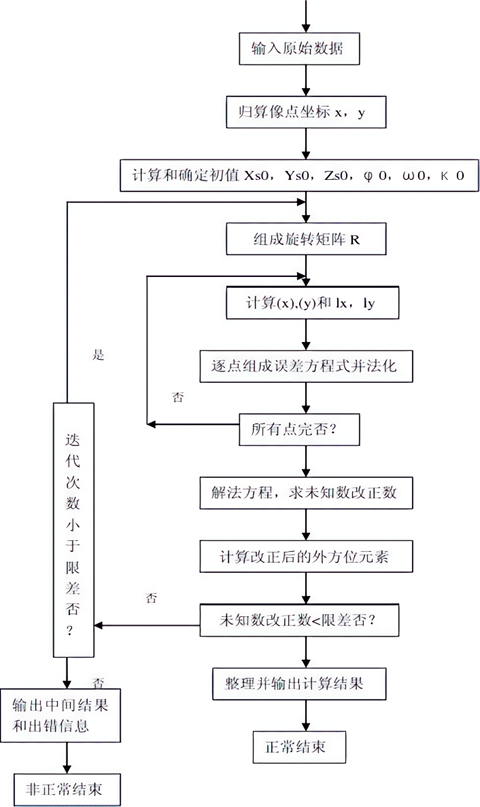
\includegraphics[width=0.6\linewidth]{figures/单像流程.png}
        \caption{单像空间后方交会流程图}
        \label{fig:原理}
    \end{figure}
    \FloatBarrier

\subsection{实习数据与代码部分}

\subsubsection{实习数据}    

摄影机主距$f=153.24mm$,$x_0=0$,$y_0=0$, 像片比例尺为1:50000,有四对点的像点坐标与相应的地面坐标如下表。
\begin{figure}[!htbp]
    \centering
    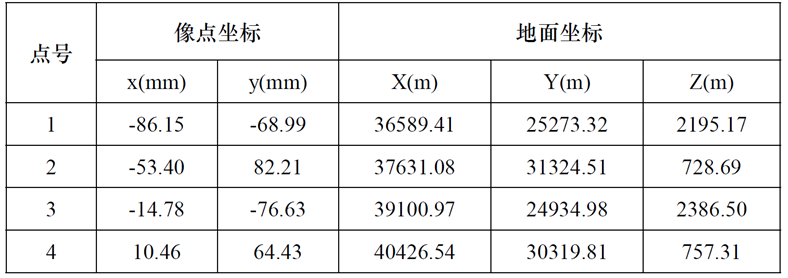
\includegraphics[width=1.0\linewidth]{figures/单像数据.png}
    \caption{单像空间后方交会数据示意}
    \label{fig:数据}
\end{figure}
\FloatBarrier

\subsubsection{实习要求}


\subsubsection{实习代码}


\subsection{实习结果与数据分析}
\subsubsection{实习结果}



%\section{定理环境}
%\begin{Theorem}
%\end{Theorem}
%
%\begin{Lemma}
%\end{Lemma}
%
%\begin{Corollary}
%\end{Corollary}
%
%\begin{Proposition}
%\end{Proposition}
%
%\begin{Definition}
%\end{Definition}
%
%\begin{Example}
%\end{Example}
%
%\begin{proof}
%\end{proof}




\section{写在最后}
\subsection{发布地址}
\begin{itemize}
    \item Github: \url{https://github.com/HMBlankcat/}
\end{itemize}




\newpage
\begin{appendices}

\section{文件列表}

\begin{table}[h]  
	\centering  
	\caption{文件列表}  
	\renewcommand{\arraystretch}{1.25} % 增加行间距  
	\begin{tabular}{c@{\hspace{20pt}}c} % 增加列间距   
		\toprule  
		文件名   & 功能描述 \\
		\midrule  
		单像空间后方交会.py & 单像空间后方交会程序代码 \\
		q2.m & 问题二程序代码 \\
		q3.m & 问题三程序代码 \\
		q4.m & 问题四程序代码 \\
		\toprule  
	\end{tabular}  
	\label{tab:文件列表}  
\end{table}  
	
	\section{代码}
	\noindent 单像空间后方交会.py
	\lstinputlisting[language=python]{code/单像空间后方交会.py}

\end{appendices}


\end{document}